\label{cap_res}

Neste capítulo, descreve-se a metodologia adotada para realizar os experimentos do \acrshort{MPM} e do \acrshort{MAR} para validação do Hare. Para tanto, os experimentos realizados buscam clarificar as seguintes perguntas:

\begin{enumerate}
    \item \label{peg1} É possível prever o próximo movimento de um ativo utilizando uma rede \acrshort{LSTM} Hiper-parametrizada?
    \item \label{peg2} A rede \acrshort{LSTM} Hiper-parametrizada é capaz de superar outros modelos presentes na literatura?
    \item \label{peg3} O algoritmo \acrshort{DDPG} é capaz de aprender a gerenciar um portfólio, com um ou mais ativos, para gerar lucros no ambiente de mercado proposto?
    \item \label{peg4} O Hare consegue gerar um rendimento maior que opções de investimento de renda fixa mais seguros?
    \item \label{peg5} O Hare consegue alocar recursos em um portfólio de forma mais lucrativa que um portfólio alocado utilizando a \acrlong{VMM}?
\end{enumerate}


\section{Metodologia}

Cada solução possui suas particularidades, e consequentemente, a avaliação de desempenho para cada solução se torna individual para cada sistema distinto \cite{jain1990art}. Com o propósito de avaliar os módulos implementados no Hare e responder as perguntas propostas, avaliações qualitativas e quantitativas foram realizadas.

O roteiro experimental valida o Hare em duas etapas: (i) validação do \acrshort{MPM} na Seção \ref{exp:mp}; e (ii) validação do \acrshort{MAR} na Seção \ref{exp:mar}. Para validar o \acrshort{MPM} realizou-se uma metodologia em três etapas: rotina de exploração de hiper-parâmetros, avaliação do desempenho dos resultados de treino e teste, e comparação com outros métodos para a resolução do problema. Posteriormente validou-se o \acrshort{MAR} analisando os modelos de cada um dos ativos e suas combinações, e os comparando com outras formas de investimento.

\subsection{Base de Dados}
\label{SEC:data-set}

Para realizar os experimentos supracitados, foi necessário a construção de uma base de dados com as informações necessárias. A base utilizada pelo Hare foi modelada manualmente através da plataforma oficial da B3\footnote{Disponível em: \url{http://www.b3.com.br/}}. A plataforma provê informações, desde 1986, sobre os ativos, tais como: nome da companhia, código de negociação, tipo de mercado, preço (abertura, fechamento, mínimo, máximo), e número de negociações feitas. Os diversos dados disponíveis na base foram tratados de acordo com a necessidade do experimento para adequá-lo à aplicação proposta. Seus tratamentos, quando realizados, são descritos dentro da seção do experimento respectivo.

\section{Experimentos do Módulo Preditor}
\label{exp:mp}

O primeiro conjunto de experimentos realizados, busca avaliar o desempenho o \acrshort{MPM} e responder as Perguntas \ref{peg1} e \ref{peg2} desta pesquisa. O processo de experimentação segue uma rotina de três passos. Começa-se explorando os hiper-parâmetros que melhor se adaptam a proposta da \acrshort{LSTM}, utilizando métodos de otimização Bayesiana fornecidos pela biblioteca Hyperopt. Posteriormente, a rede \acrshort{LSTM} calibrada com o Hyperopt, é colocada em processo de treino, avaliando sua consistência com uma série de experimentos. A rede treinada é então validada e comparada com outros modelos de aprendizado.


Para a análise dos resultados experimentais foram utilizadas as seguintes métricas: 

% clássicas de classificação, definidas nas \refEqs{eq:metric_sen}{eq:f1score}. Os valores utilizados para definições das métricas, desprendem-se de resultados de experimentos de classificação binária. Tais resultados se encaixam em um dos seguintes grupos: verdadeiro positivo VP (predição positiva correta), verdeiros negativos VN (predição negativa correta), falsos positivos FP (predição positiva incorreta), e falsos negativos FN (predição negativa incorreta). 


\equacao{eq:metric_sen}{
    \text{sensibilidade} = \frac{\text{VP}}{\text{VP} + \text{FN}}
}

\equacao{eq:metric_pre}{
    \text{precisão} = \frac{\text{VP}}{\text{VP} + \text{FP}}
}

\equacao{eq:metric_spe}{
    \text{especificidade} = \frac{\text{VN}}{\text{VN} + \text{FP}}
}

\equacao{eq:metric_acc}{
    \text{acurácia} = \frac{\text{VP} + \text{VN}}{\text{VP} + \text{VN} + \text{FP} + \text{FN}}
}

\equacao{eq:f1score}{
    \text{F1 Score} = 2 * \frac{\text{precisão} * \text{sensibilidade}}{\text{precisão} + \text{sensibilidade}}
}

Cada métrica utilizada avalia um aspecto diferente dos resultados. A \refEq{eq:metric_sen}, descreve a sensibilidade, o quão completo os resultados estão. A precisão, definida pela \refEq{eq:metric_pre}, representa o quanto os resultados da pesquisa são uteis para reprodutibilidade. A \refEq{eq:metric_spe}, descreve a especificidade, a proporção de resultados negativos corretamente identificados. A acurácia, definida pela \refEq{eq:metric_acc}, é o quão aproximado os resultados estão do valor especifico da realidade. Por último, a \refEq{eq:f1score}, descreve a métrica \textit{F1 Score}. Tal métrica leva em consideração a precisão e a sensibilidade para computar seu resultado. Seu valor representa a média harmônica entre essas métricas, onde o \textit{F1 Score} alcança a melhor precisão e sensibilidade no valor $1$ e a pior no valor $0$.

Para gerar os modelos, a base de dados foi dividida em treino, validação e teste. O treino e validação correspondem a $70\%$ dos seis meses contidos na base de dados. Os outros $30\%$ foram utilizado para a fase de teste. Todos os experimentos utilizaram uma técnica para avaliar a capacidade de generalização do modelo, denominada validação cruzada. O método escolhido para essa validação foi o \emph{Nested K-Fold}. Esse método consiste em dividir o conjunto total de dados em $k$ subconjuntos. Realizado então o treino e teste $k$ vezes. Cada vez que o $k$ é incrementado a base de treino é aumentada e treina-se no subconjunto seguinte. Neste trabalho realizou-se a validação cruzada com $k=6$, para a base de dados de seis meses.

Os experimentos foram conduzidos usando uma máquina virtual Linux hospedada na plataforma \textit{Google Cloud}. As máquinas foram fornecidas com 4 CPUs e 3.8 GB de memória principal.

\subsection{Pré Processamento da Base}

O \acrshort{MPM} do Hare utiliza uma base de dados de um semestre para treino, validação e teste. Foram usados os seguintes ativos para compor o portfólio do agente: VALE3, PETR3 e ABEV3. Além disso, utilizou-se o preço de fechamento da base de dados por ser uma reflexão de todos os movimentos do dia no mercado. Realizou-se então uma filtragem da base com apenas o preço de fechamento nos seis primeiros meses de 2014 para cada um dos ativos no portfólio. No entanto, o preço de fechamento foi submetido a um processo de normalização, utilizando uma abordagem \textit{Min-Max}, colocando os preços em intervalo de 0 a 1. 

Em experimentos iniciais observou-se que a quantidade de dados não era o suficiente para que a predição do modelo não fosse afetada pelos \emph{outliers}\footnote{Dados que se diferenciam drasticamente de todos os outros da base, pontos fora da curva.}. Como solução para tratar esses ``pontos fora da curva'', uma abordagem de duplicação dos dados foi efetuada, introduzindo a média entre dois valores consecutivos nos dados históricos. Sendo assim, a série histórica apresenta mais dados, sem variações bruscas e sem perder seu comportamento original. 

Para completar a base de dados para os experimentos do modelo preditor, realizou-se a criação de rótulos indicadores de movimento do mercado, que atendam às necessidades dos modelos de treinamento. Os rótulos foram criados utilizando uma abordagem discreta para cada ativo, em cada passo de tempo. Tal abordagem foi escolhida pois prever se um ativo vai ganhar ou perder valor é uma tarefa com maior probabilidade de acurácia do que prever o seu valor real. Sendo assim, os rótulos são determinados como $0$ caso o preço de fechamento do dia foi menor que a média da janela de dias anteriores, ou como $1$ caso o contrário. 

\subsection{Hiper-parametrização do Modelo}
\label{exp:hyper}

Com a base de dados preparada, pode-se começar a primeira fase experimental com a exploração dos hiper-parâmetros. A maioria dos algoritmos de aprendizado possuem um conjunto de variáveis previamente definidas antes do início do processo de treinamento, tais variáveis são os chamados de hiper-parâmetros. A escolha correta dos mesmos pode alterar significativamente o desempenho de um modelo. Portanto, otimizá-los de forma correta se torna um ponto essencial no processo de modelagem.

A metodologia de calibragem dos hiper-parâmetros é realizada em duas etapas. Começando com uma rotina de exploração de hiper-parâmetros utilizando métodos de otimização Bayesiana.

\subsubsection{Metodologia de Hiper-parametrização}

A rede \acrshort{LSTM} possui diferentes valores de hiper-parâmetros para cada processo de modelagem. Nesse trabalho, foram selecionados quatro parâmetros da \acrshort{LSTM} baseado nas calibrações que \textcite{random_forest_macroeconomic, ga_optimized_lstm} realizaram. \textcite{ga_optimized_lstm} calibram a janela de tempo e número de unidades \acrshort{LSTM} que seus modelos possuem. Por outro lado, \textcite{random_forest_macroeconomic} clarificam a importância dos algoritmos de otimização durante o processo de treinamento. Baseando-se nesses dois trabalhos foram escolhidos então os seguintes parâmetros a serem calibrados: janela de tempo, unidades \acrshort{LSTM}, algoritmos de otimização e o \textit{batch size}.

Tendo selecionado o conjunto de hiper-parâmetros a serem explorados, a biblioteca Hyperopt\footnote{Disponível em \url{https://github.com/hyperopt/hyperopt}} foi utilizada na aplicação dos métodos de otimização. Hyperopt é uma biblioteca em \textit{Python} que implementa um algoritmo denominado, Otimização Sequencial Baseada em Modelo (SMBO), também conhecido como otimização Bayesiana. O SMBO é aplicável em situações que a minimização do valor para alguma função $f(x)$ possui um alto custo devido à complexidade do método de avaliação. Tal método utiliza um algoritmo de busca, para determinar o conjunto de hiper-parâmetros, através de interações denominadas ensaios. 

A biblioteca Hyperopt realiza sua otimização, baseando-se em três características principais a serem definidas pelo usuário: (i) uma função objetivo; (ii) um algoritmo de busca\footnote{No período em que esse trabalho foi realizado, a biblioteca oferecia apenas duas opções: Busca aleatória e o algoritmo \acrfull{TPE}.}; e (iii) o espaço de busca utilizado pelo o algoritmo. Definido estas características, a seleção de valores é utilizada para encontrar o melhor conjunto de hiper-parâmetros para o modelo.

\subsubsection{Resultados da Hiper-parametrização}

A condução dos experimentos começou pela utilização da biblioteca Hyperopt, com o intuito de descobrir os melhores hiper-parâmetros para o modelo \acrshort{LSTM} proposto. A realização deste experimento necessita, no entanto, das definições das características de funcionamento do Hyperopt. Neste trabalho, definiu-se tais características da seguinte forma: (i) a função objetivo selecionada foi o \textit{F1 Score} retornado pelo modelo \acrshort{LSTM}, previamente apresentado na \refEq{eq:f1score}; (ii) o algoritmo de busca escolhido foi o \acrshort{TPE}; e (iii) o espaço de busca selecionado são os valores escolhidos para serem explorados para cada um dos parâmetros previamente apresentados, definidos na \refTab{tab:params}. 

\tabela{Parâmetros utilizados nos experimentos exploratórios}{tab:params}{|l|l|l|l|l|l|l|}{
\hline
Batch Size & 1    & 2   & 32      & 64  & 128 & 256 \\ \hline
Unidades LSTM & 1    & 50  & 80      & 100 & 150 & 200 \\ \hline
Janelas  & 1    & 3   & 6       & 9   & 12  & --     \\ \hline
Otimizadores   & Adam & SGD & RMSprop &  --   & --  & --    \\ \hline
}

Foram realizados três experimentos do Hyperopt, um para cada ativo no portfólio (PETR3, VALE3, ABEV3). Cada experimento foi realizado com 1000 ensaios para um ativo específico, utilizando como dado de entrada o preço de fechamento de cada dia útil do primeiro semestre de 2014. O processo de treinamento foi feito com processos paralelos, e um histórico foi gerado para permitir futuras análises das escolhas de parâmetros feita pelo algoritmo. Os resultados de cada experimento, com os melhores parâmetros encontrados para cada ativo, são apresentados na \refTab{tab:best-params}.

\tabela{Melhor conjunto de parâmetros encontrados para cada ativo}{tab:best-params}{l|l|l|l|}{
\cline{2-4}
                                    & VALE3   & PETR3   & ABEV3   \\ \hline
\multicolumn{1}{|l|}{Batch Size}    & 2       & 2       & 128     \\ \hline
\multicolumn{1}{|l|}{Unidades LSTM}   & 200     & 80      & 1       \\ \hline
\multicolumn{1}{|l|}{Janelas}    & 6       & 9       & 6       \\ \hline
\multicolumn{1}{|l|}{Otimizadores}     & RMSprop & RMSprop & Adam    \\ \hline
\multicolumn{1}{|l|}{Melhor F1 Score} & 0.78781 & 0.83006 & 0.65109 \\ \hline
}

Com os resultados obtidos, foi observado a necessidade de existir um modelo específico para cada ativo, dado que seus hiper-parâmetros são diferentes e possivelmente a forma que o modelo analisa os padrões da série temporal também é diferente. Os resultados obtidos no estudo dos hiper-parâmetros para o ativo da VALE3 mostram que sua melhor pontuação de $0.7878$, é resultado da combinação de um \textit{batch size} de 2, $200$ unidades LSTM, $6$ dias de janela e a utilização do otimizador RMSprop. Para o caso do ativo PETR3 a maior pontuação obtida foi de $0.83006$ sendo resultante da combinação de $2$ de \textit{batch size}, $80$ unidades \acrshort{LSTM}, $9$ dias de janela e \textit{RMSprop} como otimizador. Por último, o ativo ABEV3, obteve um \textit{F1 Score} de apenas $0.65109$, com $128$ de \textit{batch size}, $1$ unidade \acrshort{LSTM}, $6$ dias de janela, e Adam como otimizador.

Além de observar os melhores resultados obtidos através do Hyperopt, uma análise mais aprofundada foi realizada para entender o comportamento do algoritmo para cada ativo, os resultados são apresentados nas \refFigs{hyperopt_petr}{hyperopt_abev}. A figura da esquerda apresenta quatro histogramas, um para cada hiper-parâmetro, com os valores do parâmetro e quantidade de vezes que cada valor foi selecionado pelo algoritmo do Hyperopt. Na figura da direita é apresentado o valor da função objetivo escolhida, \emph{F1 Score}, durante os 1000 ensaios do algoritmo. Para auxiliar a visualização é adicionado um ajuste baseado em um polinômio de primeiro grau, para traçar uma reta capaz de representar a tendência dos dados.

A \refFig{hyperopt_petr}, representa os resultados do experimento para os ativos PETR3. Quando analisado seu histograma, pode-se observar que os parâmetros mais selecionados, com exceção da janela, não correspondem aos melhores parâmetros escolhidos pelo Hyperopt demonstrados na \refTab{tab:best-params}. O que pode indicar que o algoritmo de seleção dos hiper-parâmetros busca priorizar a exploração de valores que obtiveram resultados piores, do que aproveitar de primeira os melhores resultados encontrados. No entanto, mesmo os melhores parâmetros escolhidos não corresponderem a quantidade, observa-se através do ajuste de polinômio que o \emph{F1 Score} converge para resultados melhores.

\figura[ht]{img/hyperopt/PETR3}{Histograma de parâmetros selecionados e progressão do \textit{F1 Score} no ativo PETR3}{hyperopt_petr}{width=1\linewidth}%

\figura[ht]{img/hyperopt/VALE3}{Histograma de parâmetros selecionados e progressão do \textit{F1 Score} no ativo VALE3}{hyperopt_vale}{width=1\linewidth}%

Por outro lado, ao observar a \refFig{hyperopt_vale}, nota-se no histograma, que o \textit{batch size}, unidades \acrshort{LSTM} e otimizadores mais selecionados correspondem as escolhas de melhores parâmetros do Hyperopt para o modelo da VALE3, divergindo apenas com a janela. Tal comportamento pode ser justificado pelo algoritmo de exploração de parâmetros, encontrar em sua maioria das vezes, valores de \emph{F1 Score} satisfatórios. Observa-se também que o ativo VALE3 provou possuir o modelo mais consistente, com base no \emph{F1 Score} em comparação com os ativos PETR3 e ABEV3.


Similarmente, o ativo ABEV3, apresentado na \refFig{hyperopt_abev}, difere os valores mais selecionados dos melhores valores encontrados pelo tamanho da janela e adicionalmente pelo \textit{batch size}. Ao analisar o \emph{F1 Score} deste experimento, observa-se que não somente foi o pior obtido, como também foi bem abaixo dos outros valores. Este comportamento pode ser um reflexo da incerteza do inerente ao primeiro ano do ativo na bolsa, que haveria trocado seu código e seus papéis após uma reestruturação societária no final de 2013.

\figura[ht]{img/hyperopt/ABEV3}{Histograma de parâmetros selecionados e progressão do \textit{F1 Score} no ativo ABEV3}{hyperopt_abev}{width=1\linewidth}%

Portanto, nota-se que os resultados obtidos sempre demonstram um aumento da inclinação na função objetivo dos três ativos. Sendo assim, observando a representação do \textit{F1 Score} pelo polinômio de primeiro grau apresentado, nota-se que de fato há um aumento no valor com o passar dos ensaios, demonstrando que o processo de hiper-parametrização apresenta melhorias. Conclui-se também que os parâmetros mais selecionados não necessariamente indicam que farão parte do grupo de melhores parâmetros ao final do experimento, o que pode indicar a tentativa do algoritmo de explorar novas combinações.

\subsection{Treinamento e Desempenho do Modelo}
\label{exp:train}

Após a hiper-parametrização dos modelos propostos, conduziu-se experimentos para treinar os melhores modelos. Tais experimentos de treino levam em consideração o comportamento da função de perda e da consistência de acurácia para diferentes janelas de tempo. 

Para cada ativo, um novo experimento foi executado utilizando os melhores resultados de hiper-parâmetros fornecidos pelos testes realizados anteriormente. O experimento consiste em um K-Fold de validação cruzada, com $k=6$, para cada janela de tempo apresentada na \refTab{tab:params}. Os resultados são apresentados nas \refFigs{train_petr}{train_abev}. 
% O gráfico da esquerda apresenta o comportamento da função de perda em 5000 épocas de treino. No topo direito, o gráfico de caixas mostra a distribuição e valores discrepantes da acurácia obtida para cada janela de tempo. Na direita da figura, se apresenta a matriz de confusão para os modelos com janela que obtiveram o melhor desempenho, e os valores das métricas analisadas. A matriz de confusão permite avaliar o modelo preditivo, obtendo informações sobre o comportamento das predições. Os resultados buscados na matriz são aqueles em que o rótulo previsto possui o mesmo valor do rótulo verdadeiro, o que indica uma previsão verdadeira de ganho no preço do ativo em caso de $1$, e uma previsão verdadeira de perda no preço do ativo em caso de $0$. Caso o rótulo previsto, não entre em acordo com o rótulo verdadeiro, é dito que houve um falso negativo ou falso positivo.

A \refFig{train_petr} demonstra o treinamento do ativo da PETR3 que apresentou o maior \emph{F1 Score}, de $0.83006$, na hiper-parametrização. Os resultados obtidos demonstram que a janela pode impactar de forma significante o modelo. Observa-se que janelas de tamanho $1$ e $3$ são as de piores desempenho. Já as janelas $6$, $9$ e $12$ apresentam resultados melhores. Dentre estes, a janela de tamanho $6$ foi escolhida para ser utilizada. Apesar da dispersão do modelo ser maior que o de tamanho $12$, seu limite superior é bem maior, chegando inclusive a $100\%$ em algumas situações. Além de apresentar também um limite inferior bem maior que a janela de tamanho $9$. Outra característica também importante para a seleção deste tamanho de janela foi a mediana, que é a mais simétrica entre as janelas. Considerando então a janela de tamanho $6$, seus resultados de predição são apresentados na matriz de confusão. Com as predições realizadas pelo modelo, se obteve as seguintes métricas: acurácia de $0.803$, especificidade de $0.7939$, precisão de $0.8$ e sensibilidade de $0.812$. Observa-se que todas as métricas apresentam valores altos, portanto o modelo gerado possui $81,2\%$ de resultados completos, é $80\%$ reprodutível, possui uma taxa de acerto das predições de $80,3\%$ e identifica corretamente $79\%$ dos decréscimos de valor no preço de um ativo.

\figura[ht]{img/train/PETR3}{Função de perda e matriz de confusão do ativo PETR3}{train_petr}{width=.9\linewidth}

%Em particular, os resultados da VALE3, demostrados na \refFig{train_vale}, apresentam modelos mais concisos, com menor dispersão, que os apresentados no modelo da PETR3. Além de mostrar também, um valor de mediana de melhor acurácia na maioria das janelas. Assim como na PETR3, as janelas de $1$ e $3$ podem ser desconsideradas por apresentarem novamente resultados piores. Dentre as janelas $6$, $9$ e $12$, a janela de tamanho $6$ foi a escolhida por apresentar o maior limite inferior, e possuir a menor dispersão entre os resultados. A matriz de confusão foi então criada com base no treinamento do modelo com o tamanho de janela $6$. Novamente, com as predições realizadas pelo modelo obteve-se os valores das seguintes métricas: acurácia de $0.8144$, especificidade de $0.8794$, precisão de $0.8426$ e sensibilidade de $0.7398$. Observa-se que quase todas as métricas obtiveram resultados melhores que o modelo da PETR3, com exceção da sensibilidade. Portanto, este modelo apresenta um resultado menos completo ($73,9\%$), mas uma maior reprodutibilidade ($84,2\%$), maior taxa de acerto ($81,4\%$) e maior taxa de identificação de decréscimos ($87,94\%$).

\figura[ht]{img/train/VALE3}{Função de perda e matriz de confusão do ativo VALE3}{train_vale}{width=.9\linewidth}


Finalizando a análise do processo de treinamento, as \refFig{train_vale} e \refFig{train_abev} demonstram os resultados para os modelos da VALE3 e ABEV3, respectivamente. Os modelos para esses ativos foram os que obtiveram as menores métricas F1 Score no processo de hiper-parametrização. Entretanto, a concisão de ambos os modelos se apresentou superior aos modelos da PETR3, possuindo uma menor dispersão se compararmos janelas de tamanhos iguais. Assim como na PETR3, as janelas de tamanho 1 e 3 podem ser desconsideradas para os modelos da VALE3, e para a ABEV3, os tamanhos 1, 3 e 12 por apresentarem resultados piores. Dentre as janelas restantes o tamanho 6 foi escolhido para o modelo da VALE3, por apresentar um limite inferior menor e para o modelo da ABEV3 foi escolhido o tamanho de janela 9, por ser bastante conciso permitindo uma maior chance de reprodutibilidade. Observando-se particularmente as predições realizadas pelo modelo da VALE3 com janela de tamanho 6 obteve-se os valores das seguintes métricas: acurácia de $0.8144$, especificidade de $0.8794$, precisão de $0.8426$ e sensibilidade de $0.7398$. Observa-se que quase todas as métricas obtiveram resultados melhores que o modelo da PETR3, com exceção da sensibilidade. Portanto, este modelo apresenta um resultado menos completo ($73,9\%$), mas uma maior reprodutibilidade ($84,2\%$), maior taxa de acerto ($81,4\%$) e maior taxa de identificação de decréscimos ($87,94\%$). Por fim com os resultados então obtidos na matriz de confusão para o modelo com o tamanho de janela $9$ da ABEV3, obteve-se as métricas de análise. Os valores obtidos para acurácia ($0.8333$) e sensibilidade ($0.8871$) foram os maiores em comparação com os outros ativos. Indicando a maior taxa de acerto ($83,3\%$) e a maior completude dos resultados ($88,71\%$), resultado provavelmente proveniente da escolha do modelo mais conciso. No entanto, sua especificidade é a menor obtida com o valor de $0.7787$, o que indica que a capacidade do modelo prever uma queda do preço do ativo é de $77,8\%$. Finalizando, a precisão de $0.8029$, se apresenta com um valor parecido do modelo da PETR3, indicando a capacidade do modelo de reprodutibilidade em $80,2\%$.

%Finalizando a análise do processo de treinamento, a \refFig{train_abev} demonstra os resultados dos modelos para o ativo ABEV3. Os modelos para esse ativo, foram aqueles que obtiveram a menor métrica \emph{F1 Score} ($0.65109$) no processo de hiper-parametrização. Os resultados da acurácia por janela apresentam valores inferiores aos outros ativos nas janelas $1$, $3$ e $12$, além de serem bem piores que a janelas $6$ e $9$, sendo assim, descartadas. Dentre as janelas restantes, observa-se que o limite inferior da acurácia é semelhantes, e a janela de tamanho $6$ é a que chega a obter maiores acurácias. No entanto, pelo modelo de tamanho de janela $9$ ser bastante conciso, é provável que este possa ter uma reprodutibilidade maior em generalizar casos fora dos dados separados para treino e teste. Com os resultados então obtidos na matriz de confusão para o modelo com o tamanho de janela $9$, obteve-se as métricas de análise. Os valores obtidos pra acurácia ($0.8333$) e sensibilidade ($0.8871$) foram os maiores em comparação com os outros ativos. Indicando a maior taxa de acerto ($83,3\%$) e a maior completude dos resultados ($88,71\%$), resultado provavelmente proveniente da escolha do modelo mais conciso. No entanto, sua especificidade é a menor obtida com o valor de $0.7787$, o que indica que a capacidade do modelo prever uma queda do preço do ativo é de $77,8\%$. Finalizando, a precisão de $0.8029$, se apresenta com um valor parecido do modelo da PETR3, indicando a capacidade do modelo de reprodutibilidade em $80,2\%$.

\figura[ht]{img/train/ABEV3}{Função de perda e matriz de confusão do ativo ABEV3}{train_abev}{width=.9\linewidth}

Com a análise dos resultados das \refFigs{train_petr}{train_abev} pode ser notado a importância do parâmetro da janela de tempo, podendo impactar significativamente a acurácia do modelo. As janelas com melhor desempenho apresentaram valores altos nas matrizes de confusão mostrando a eficiência na escolha dos hiper-parâmetros. Avaliando as matrizes de confusão, percebe-se que todos os modelos apresentaram resultados de predição satisfatórios. As métricas e o tamanho de janela resultantes para os modelos são resumidos na \refTab{tab:resumo}. Portanto, esses resultados demostram a viabilidade do uso de modelos \acrshort{LSTM} hiper-parametrizados na predição do movimento de ativos no Hare.

\tabela{Resumo dos resultados obtidos do \acrshort{MPM} para os ativos selecionados}{tab:resumo}{l|c|c|c|}{
\cline{2-4}
                                     & \multicolumn{1}{l|}{PETR3} & \multicolumn{1}{l|}{VALE3} & \multicolumn{1}{l|}{ABEV3} \\ \hline
\multicolumn{1}{|l|}{Janela}         & 6                          & 6                          & 9                          \\ \hline
\multicolumn{1}{|l|}{Acurácia}       & 80,30\%                    & 81,44\%                    & \textbf{83,33\%}           \\ \hline
\multicolumn{1}{|l|}{Precisão}       & 80\%                       & \textbf{84,26\%}           & 80,29\%                    \\ \hline
\multicolumn{1}{|l|}{Sensibilidade}  & 81,20\%                    & 73,98\%                    & \textbf{88,71\%}           \\ \hline
\multicolumn{1}{|l|}{Especificidade} & 79,39\%                    & \textbf{87,94\%}           & 77,87\%                    \\ \hline

}

Em seguida, utilizando os melhores modelos, uma análise real de mercado foi realizada. O objetivo é entender o comportamento das predições de cada um dos ativos, validando as métricas encontradas nos experimentos anteriores. Os resultados são apresentados nas \refFigs{petr_pred}{abev_pred}. Os gráficos apresentam a variação do preço de fechamento do ativo ao longo do tempo (linha rosa) e a variação do preço médio na janela de tempo selecionada para o ativo (linha azul). Os marcadores presentes na linha azul representam as predições de preço em relação à média de dias anteriores, a seta verde para cima representa que a predição de aumento foi correta, enquanto a seta vermelhar para baixo representa a predição correta. Predições incorretas são representadas por um $x$ verde ou vermelho para um aumento ou decréscimo respectivamente.

\figura[th]{img/predictions/PETR3.pdf}{Predições do ativo PETR3}{petr_pred}{width=1\linewidth}%
\figura[th]{img/predictions/VALE3.pdf}{Predições do ativo VALE3}{vale_pred}{width=1\linewidth}%
\figura[th]{img/predictions/ABEV3.pdf}{Predições do ativo ABEV3}{abev_pred}{width=1\linewidth}%

Como se pode observar a acurácia foi satisfatória para todos os ativos avaliados. No pior caso, a acurácia foi de $82\%$ para o ativo da VALE3 (\refFig{vale_pred}). Em contraste, o ativo PETR3 obteve $92\%$ (\refFig{petr_pred}) de acerto, seguindo pelo ABEV3 com $94\%$ (\refFig{abev_pred}). Tais resultados demonstram a eficiência do modelo \acrshort{LSTM} hiper-parametrizado proposto, e respondem à Pergunta \ref{peg1} proposta. Observa-se também nos resultados que a maioria dos erros preditivos acontecem em transições de movimento, o que pode ser considerado uma possível limitação da \acrshort{LSTM}. Portanto, modelos aplicados a ativos de alta volatilidade, podem se tornar um desafio extra para o \acrshort{MPM}, reforçando assim a necessidade de um modulo que estude as características fundamentais para analisar riscos.


\subsection{Comparação com Modelos de Base}
\label{exp:base}

Mesmo com o modelo \acrshort{LSTM} proposto apresentando resultados promissores, foi realizada uma análise comparativa com outros modelos tradicionais de aprendizado de máquina, sendo eles: (i) \acrshort{KNN}; (ii) \acrshort{SVM}; (iii) \acrshort{RNN}; e (iv) \acrshort{GRU}. Além disso, é realizada uma análise comparativa com uma rede \acrshort{LSTM} sem o processo de hiper-parametrização para identificar a diferença entre os modelos. Os modelos selecionados foram submetidos a um experimento similar ao realizado para a \acrshort{LSTM} hiper-parametrizada, utilizando a série histórica dos seis primeiros meses de 2014 do ativo PETR3. O ativo PETR3 foi selecionado para o método comparativo entre os modelos, pois obteve o pior desempenho em relação aos outros ativos, como apresentado na \refTab{tab:resumo}.

Tendo em vista que o experimento é uma comparação de algoritmos, não seria razoável comparar um modelo hiper-parametrizado, com modelos não parametrizados. Os modelos comparativos precisam possuir também algum tipo de parametrização para se mostrarem viáveis a aplicação. O modelo \acrshort{SVM} foi parametrizado em relação ao \emph{kernel} RBF, calibrando o parâmetro de regularização C para permitir que hiperplano fique mais suave evitando situações de sobreajuste, e um parâmetro gamma que define até que ponto a influência de um único exemplo de treinamento atinge. No caso do \acrshort{KNN} os experimentos foram realizados com valor de $k$ fixado em 1. No entanto, para adaptá-lo ao problema de séries temporais, o modelo foi parametrizado com a métrica de distância \acrfull{DTW}. Para as redes neurais profundas, \acrshort{RNN}, \acrshort{GRU} e \acrshort{LSTM} a janela de tempo de tamanho $6$, igual à do modelo proposto, foi utilizada. As redes foram todas treinadas com uma unidade por um total de 5000 épocas. A \refTab{tab:comparacao} resume os resultados encontrados por todos os modelos comparativos e o resultado do modelo proposto, para o ativo PETR3.


\tabelaBig{Resumo comparativo do \acrshort{MPM} proposto com métodos selecionados}{tab:comparacao}{l|c|c|c|c|c|c|}{
\cline{2-7}
                               & SVM     & KNN     & RNN     & LSTM             & GRU     & LSTM Proposta    \\ \hline
\multicolumn{1}{|l|}{Acurácia} & 55,17\% & 55,17\% & 67,74\% & 70,97\%          & 41,94\% & \textbf{80,30\%} \\ \hline
\multicolumn{1}{|l|}{Precisão} & 47,73\% & 47,73\% & 87,50\% & \textbf{93,33\%} & 83,33\% & 80\%             \\ \hline
\multicolumn{1}{|l|}{Sensibilidade}      & \textbf{87,50\%} & \textbf{87,50\%} & 63,64\% & 63,64\%          & 22,73\%          & 81,20\%          \\ \hline
\multicolumn{1}{|l|}{Especificidade}     & 32,35\%          & 32,35\%          & 77,78\% & \textbf{88,89\%} & \textbf{88,89\%} & 79,39\%          \\ \hline
}


%%\tabelaBig{Resumo comparativo do \acrshort{MPM} proposto com métodos selecionados}{tab:comparacao}{l|c|c|c|c|c|c|}{
%%\cline{2-7}
%%                               & SVM     & KNN     & RNN     & LSTM             & GRU     & LSTM Proposta    \\ \hline
%%\multicolumn{1}{|l|}{Acurácia} & 55,17\% & 55,17\% & 67,74\% & 70,97\%          & 41,94\% & \textbf{80,30\%} \\ \hline
%%\multicolumn{1}{|l|}{Precisão} & 47,73\% & 47,73\% & 87,50\% & \textbf{93,33\%} & 83,33\% & 80\%             \\ \hline
%%\multicolumn{1}{|l|}{Sensibilidade}      & \textbf{87,50\%} & \textbf{87,50\%} & 63,64\% & 63,64\%          & 22,73\%          & 81,20\%          \\ \hline
%%\multicolumn{1}{|l|}{Especificidade}     & 32,35\%          & 32,35\%          & 77,78\% & \textbf{88,89\%} & \textbf{88,89\%} & 79,39\%          \\ \hline
%%\multicolumn{1}{|l|}{Média das Métricas} & 55,68\%          & 55,68\%          & 74,78\% & 79,20            & 59,22\%          & \textbf{80,22\%} \\ \hline
%%}

Iniciando a análise pelos métodos clássicos, a \acrshort{SVM}\footnote{Parametrizado com $C = 0.1$ e $\gamma = 1$} e o \acrshort{KNN}\footnote{Parametrizado utilizando a métrica \acrshort{DTW}} obtiveram resultados semelhantes, com uma acurácia de $55\%$, muito abaixo do modelo proposto. Acredita-se que tal resultado pode ser fruto do desequilíbrio entre as classes de alta e baixa na série temporal. Em relação aos resultados das redes neurais, pode-se observar que o modelo da \acrshort{LSTM}, mesmo sem hiper-parametrização, se sobressai perante os demais em todas as métricas, empatando somente na sensibilidade com o modelo da \acrshort{RNN}. Em relação ao modelo \acrshort{LSTM} proposto, apesar de não apresentar o melhor resultado para todos as métricas, é o que apresenta a melhor acurácia, com vantagem de aproximadamente $10\%$, além da média de suas métricas ser relativamente melhor que a dos outros modelos.

Portanto, é visível que o modelo proposto, excede o desempenho de outros modelos de aprendizagem de máquina. Observa-se também que a hiper-parametrização aumenta consideravelmente o resultado do modelo \acrshort{LSTM} gerado, respondendo à Pergunta \ref{peg2} deste trabalho. Com esses resultados encerra-se os experimentos relacionados ao \acrshort{MPM}. Faltando então analisar o desempenho de como o \acrshort{MAR} trata as informações previstas.

\section{Experimentos de Alocação de Recursos}
\label{exp:mar}

Após a realização dos experimentos do \acrshort{MPM}, realizou-se os experimentos do \acrshort{MAR} focando responder as Perguntas \ref{peg3}, \ref{peg4} e \ref{peg5}. Finalizando assim a validação da proposta de um sistema de investimento autônomo, racional baseado em agentes, capaz de lidar com predições e alocações de recursos de forma apropriada. 

A proposta definida para a criação deste módulo, envolve a utilização do algoritmo \acrshort{DDPG} de aprendizagem com reforço, junto com o ambiente simulado da B3 criado. A versão implementada do algoritmo da \acrshort{DDPG} possui uma série de hiper-parâmetros a serem adaptados para a proposta. Dentre esses, citam-se os que foram utilizados: tamanho do buffer de repetição, fator de desconto, taxa de aprendizagem da política, taxa de aprendizagem do Q-Valor, \emph{batch size}, passos iniciais, ruído, tamanho da camada escondida da rede ator-critico, e camadas de ativação da rede ator crítico. 

O algoritmo do \acrshort{DDPG} foi então calibrado de forma empírica, com valores que apresentaram resultados satisfatórios em experimentos prévios realizados. Os valores encontrados na calibração são resumidos na \refTab{tab:ddpg_params}

\tabela{Parâmetros utilizados no treinamento do \acrshort{DDPG}}{tab:ddpg_params}{|l|l|}{
\hline
\textbf{Parâmetro}                     & \multicolumn{1}{c|}{\textbf{Valor Selecionado}} \\ \hline
Épocas                                 & 200                                             \\ \hline
Passos por Época                       & 1000                                            \\ \hline
Taxa de Aprendizagem da Política       & 0.0005                                          \\ \hline
Taxa de Aprendizagem do Q-Valor        & 0.0001                                          \\ \hline
Buffer de Repetição                    & 500.000                                         \\ \hline
Batch Size                             & 100                                             \\ \hline
Passos Iniciais                        & 10                                              \\ \hline
Ruído                                  & 1.0                                             \\ \hline
Tamanho da Camada Escondida            & (16, 16)                                        \\ \hline
Função de Ativação da Camada Escondida & ReLU                                            \\ \hline
Função de Ativação da Saída            & Tanh                                            \\ \hline
Episódios de Teste                     & 10                                              \\ \hline
}

Assim como nos experimentos do \acrshort{MPM}, os experimentos realizados no \acrshort{MAR} utilizaram dados do primeiro semestre de 2014. Para evitar a propagação do erro no modelo de treinamento, os rótulos de predição verdadeiros foram alimentados, não utilizando a predição realizada pelo \acrshort{MPM}, nem pelo \acrshort{MGR}. Os experimentos foram realizados de forma crescente em complexidade, realizando primeiro experimentos individuais, e finalizando com o experimento do portfólio. Como os dados do \acrshort{MGR} são fontes de uma abordagem sintética, com o proposito primário de auxiliar no entendimento do funcionamento do Hare, os experimentos aqui realizados não os levam em consideração. No entanto, um experimento extra, foi realizado e está descrito no Apêndice \ref{apendice:extra} deste trabalho.

A análise dos resultados é realizada de forma comparativa com a rentabilidade da poupança\footnote{Informações retiradas de: \url{http://www.yahii.com.br/poupanca.html}} e do \acrfull{CDI}\footnote{Informações retiradas de: \url{http://www.yahii.com.br/cetip13a21.html}}, os quais renderam $3,35\%$ e $4,87\%$ respectivamente no período avaliado. Outra comparação realizada foi com o rendimento do portfólio caso o investidor tenha realizado uma estratégia \emph{buy and hold}, onde o investidor decide comprar um ativo e ``segura-lo'' para o longo prazo, de forma a se beneficiar com os rendimentos e valorizações que o papel por ventura apresentará no futuro.

\subsection{Alocação dos Ativo Individuais}

O primeiro tipo de experimento realizado pelo \acrshort{MAR} foi utilizando ativos individuais, para analisar como a \acrshort{DDPG} funcionaria em ambientes mais simples. Desta forma três experimentos foram realizados, um para cada ativo. Cada experimento utilizou o melhor parâmetro de janela encontrado pelo \acrshort{MPM} e considerou R\$$10.000,00$ de investimentos iniciais. Os modelos foram treinados com 200 épocas e 10 episódios de teste por época. As métricas utilizadas foram o retorno e o lucro obtido no treino e no teste, as ações tomadas, o comportamento das funções de perda, e o comportamento do Q-Valor. Nesta seção descreve-se o resumo dos resultados encontrados, uma análise completa contendo todos os gráficos obtidos em treino se encontra disponível no Apêndice \ref{apendice:ativos}.

Em relação ao retorno obtido no treinamento e no teste, observou-se que mesmo tendo lucros o retorno se mantinha majoritariamente negativo, tal resultado pode ser reflexo da formulação da função de recompensa. O valor de retorno final mais alto em teste foi de $82.272$ para Petrobras, enquanto o menor foi da Ambev de $-68.70$. Continuando a análise do treinamento, observou-se que as funções de perda da política e do Q-Valor convergiram, mas não chegaram próximo de 0, o que pode indicar que o \acrshort{DDPG} convergiu para um mínimo local ou para uma situação de \emph{deadlock} \cite{matheron2019problem}. Partindo então para a análise do teste, percebeu-se que muitas vezes o agente realizaria uma ação especifica, ao invés de alternar entre compras, vendas e esperas\footnote{Vale enfatizar que nem toda ação selecionada é de fato executa. Se uma ação de compra é requerida, e o agente não possui a quantidade de dinheiro para comprar o ativo, a mesma não vai ser executada, e o agente recebe uma punição pela ação realizada de forma incorreta. A mesma lógica se aplica de forma similar para as vendas.}. No entanto, mesmo com esse comportamento, resultados satisfatórios ainda foram encontrados, obteve-se lucros de R\$$1.377,00$, R\$$603,00$, e R\$$0,00$ para os ativos PETR3, VALE3 e ABEV3 respectivamente. A \refTab{tab:res_individual} apresenta os lucros, rentabilidades e rendimentos comparativos em relação a poupança e ao CDI.

% Please add the following required packages to your document preamble:
% \usepackage{multirow}


\tabela{Resultados obtidos nos investimentos realizados pelo Hare em comparação com poupança, CDI e estratégia \emph{buy and hold}}{tab:res_individual}{cl|c|c|c|}{
\cline{3-5}
\cline{3-5}
\multicolumn{1}{l}{}                                                                                                &                                                                            & \multicolumn{1}{l|}{PETR3}   & \multicolumn{1}{l|}{VALE3}  & \multicolumn{1}{l|}{ABEV3} \\ \hline
\multicolumn{1}{|c|}{\multirow{2}{*}{\begin{tabular}[c]{@{}c@{}}Análise da Estratégia\\ Buy and Hold\end{tabular}}} & Lucro                                                                      & R\$$624,00$  & $-$R\$$957,00$   & $-$R\$$730,00$  \\ \cline{2-5} 
\multicolumn{1}{|c|}{}                                                                                              & Rentabilidade                                                              & $6,24\%$                     & $-9,57\%$                   & $-7.30\%$                  \\ \hline
\multicolumn{1}{|c|}{\multirow{4}{*}{\begin{tabular}[c]{@{}c@{}}Análise de Desempenho \\ do Hare\end{tabular}}}     & Lucro                                                                      & R\$$1377,00$ & R\$$603,00$ & R\$$0,00$  \\ \cline{2-5} 
\multicolumn{1}{|c|}{}                                                                                              & Rentabilidade                                                              & $13,77\%$                    & $6,03\%$                   & $0\%$                      \\ \cline{2-5} 
\multicolumn{1}{|c|}{}                                                                                              & \begin{tabular}[c]{@{}l@{}}Rendimento Comparado \\ à Poupança\end{tabular} & $311,04\%$                   & $80\%$                      & \textbf{-}                 \\ \cline{2-5} 
\multicolumn{1}{|c|}{}                                                                                              & \begin{tabular}[c]{@{}l@{}}Rendimento Comparado\\ ao CDI\end{tabular}      & $182,75\%$                   & $23,81\%$                   & \textbf{-}                 \\ \hline
 
}


Observa-se que os modelos da PETR3 e VALE3 encontraram resultados melhores, com uma rentabilidade de $13,77\%$ e $6,03\%$ respectivamente. Tais rentabilidades são maiores que a da poupança do CDI e de um investimento seguindo uma estratégia \emph{buy and hold}, chegando a render mais que o dobro desses investimentos para o ativo da Petrobras. Por outro lado, o modelo treinado para ABEV3 não apresenta nenhum tipo de lucro, consequentemente, não tendo rentabilidade. No entanto, observa-se que o ativo desvalorizaria $9,3\%$ no período analisado, indicando que a estratégia aprendida pelo agente, apesar de não ser ótima, consegue evitar prejuízos ao investidor.

\subsection{Alocação do Portfólio Completo}

Todos os experimentos analisados na seção anterior utilizam apenas um ativo específico, uma contradição a Teoria Moderna do Portfólio, que diz que os fatores devem ser calculados e analisados em relação ao conjunto de ativos \cite{markowitz}. Esse experimento busca então analisar o desempenho do agente com um portfólio diversificado de ativos. O portfólio foi então construído com os ativos utilizados nos experimentos anteriores (PETR3, VALE3 e ABEV3) e suas janelas respectivas. Com o propósito de aumentar a quantidade de ativos que o agente consegue investir, a quantidade de dinheiro inicial foi definida como R\$$50.000,00$. As \refFigs{all_clean_qval}{all_clean_act}, demonstram os dados obtidos em 200 épocas de experimentos. A \refFig{all_clean_qval} apresenta o comportamento do retorno médio obtido por episódios de treino e teste. Observe que diferente dos ativos individuais o retorno chega a assumir valores bem maiores, resultado consequente da maior quantidade de recursos inserida no sistema. Nota-se também que é visível a convergência do retorno médio de treinamento ao longo do treino e teste, obtendo um valor final de $404.24$ para ambos treino e teste.

\figura{img/ddpg/all/clean/return}{Portfólio - Retorno médio}{all_clean_ret}{width=.5\linewidth}

Analisa-se também o Q-Valor médio e as funções de perda do treinamento, com base nas \refFigs{ptr_clean_qval}{petr_clean_loss}. O Q-Valor alcança uma média de $230,84$, variando entre $1633,95$ a $-594,62$, enquanto as funções de perda assumem valores de $2.357,02$ e $-232.13$ para perda Q (função de aproximação do Q-Valor) e perda $\pi$ (função de aproximação da política) respectivamente. Nota-se que os valores de perda são maiores que dos ativos individuais, o que representa uma correlação entre a recompensa maior obtida, devido a maior quantidade de recursos no sistema. Apesar desses valores ainda serem extremamente altos para funções de perda, experimentos com maiores números de época não apresentaram resultados diferentes ao comportamento.

\begin{figure}[htbp]
    \centering 
    \begin{minipage}[b]{0.45\linewidth}
        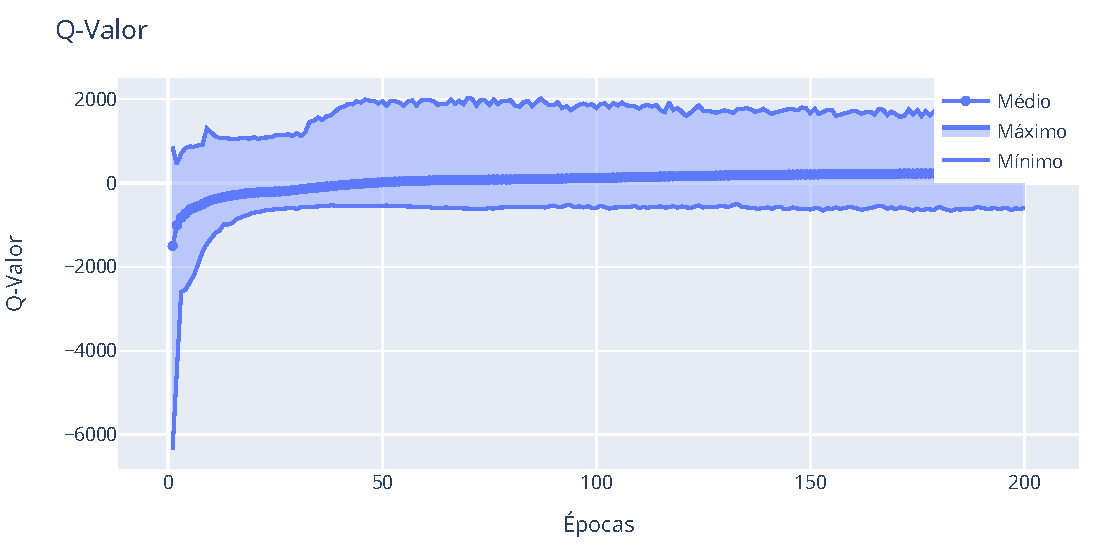
\includegraphics[width=\linewidth]{img/ddpg/all/clean/qval}
        \caption{Portfólio - Comportamento do QValor.} 
        \label{all_clean_qval}
    \end{minipage}
    \quad
    \begin{minipage}[b]{0.45\linewidth}
        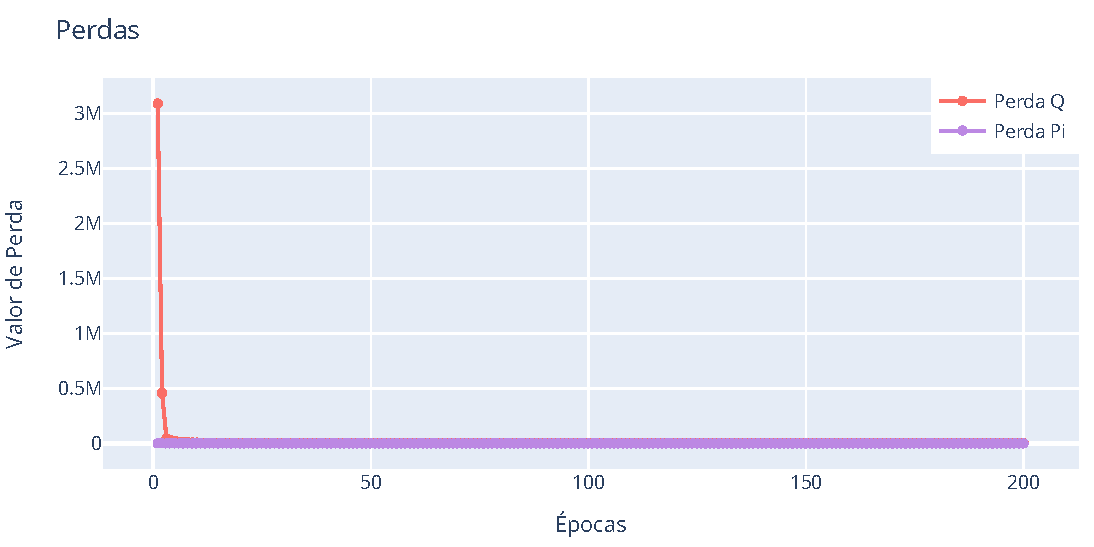
\includegraphics[width=\linewidth]{img/ddpg/all/clean/loss}
        \caption{Portfólio - Comportamento das funções de perda.}
        \label{all_clean_loss}
    \end{minipage}
\end{figure}

Em relação ao lucro obtido, nota-se na \refFig{all_clean_ptrain}, que durante o treino se obteve uma alta dispersão de valores, incluindo um lucro de R\$$23.860,00$ em um dos episódios. Novamente, no entanto, o algoritmo não explora essas recompensas maiores. Esse comportamento também foi observado nos outros experimentos, o estudo do mesmo abre possibilidades para trabalhos futuros que podem ser capazes de melhorar significantemente os modelos. Se o agente tivesse explorado o melhor lucro encontrado, teria obtido um rendimento de aproximadamente $47\%$ no período, quase $8\%$ ao mês.  

\figura[htbp]{img/ddpg/all/clean/profit_train}{Portfólio - Lucro em treino}{all_clean_ptrain}{width=.5\linewidth}

Quando o resultado do lucro é observado em teste (\refFig{petr_clean_profit}), percebe-se oscilações menores (por não conter ruído em suas ações), e nota-se que também não é explorada a política com maior lucro encontrada. No entanto, mesmo com essas limitações presentes no modelo proposto, ao final do treinamento obteve-se um lucro médio de R$\$5.874$, realizando ações majoritariamente de venda, comprando algumas vezes, e nunca realizando a ação de espera (veja a \refFig{all_clean_act}). Observa-se que a ação de espera raramente é selecionada em experimentos, sendo de ativos individuais ou do portfólio completo, esse comportamento provavelmente é fruto da função de recompensa, cabendo a trabalhos futuros investigar como adaptar a função para melhorar o sistema.

\begin{figure}[htbp]
    \centering 
    \begin{minipage}[b]{0.45\linewidth}
        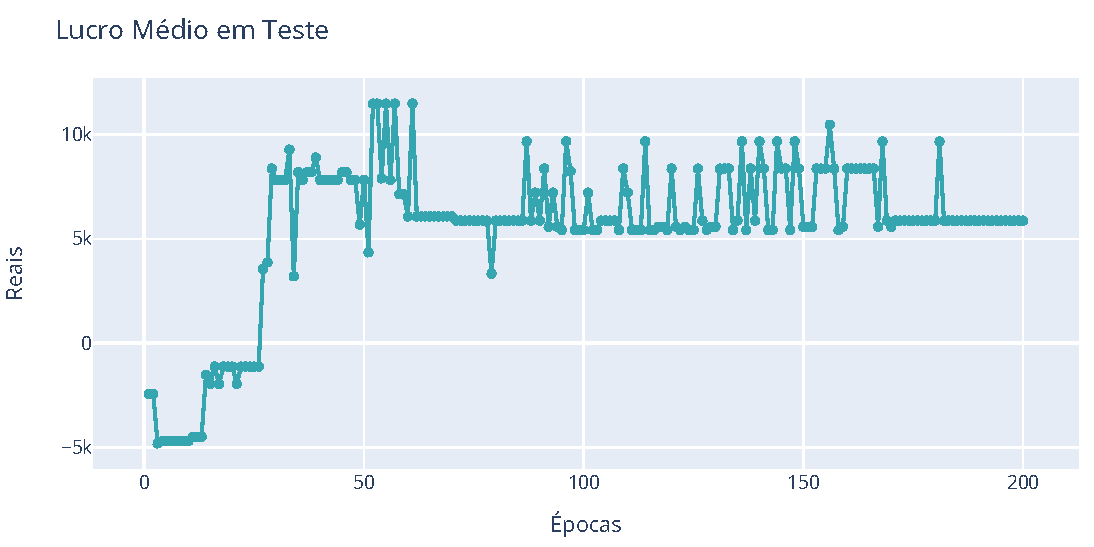
\includegraphics[width=\linewidth]{img/ddpg/all/clean/profit}
        \caption{Portfólio - Lucro médio em teste.} 
        \label{all_clean_profit}
    \end{minipage}
    \quad
    \begin{minipage}[b]{0.45\linewidth}
        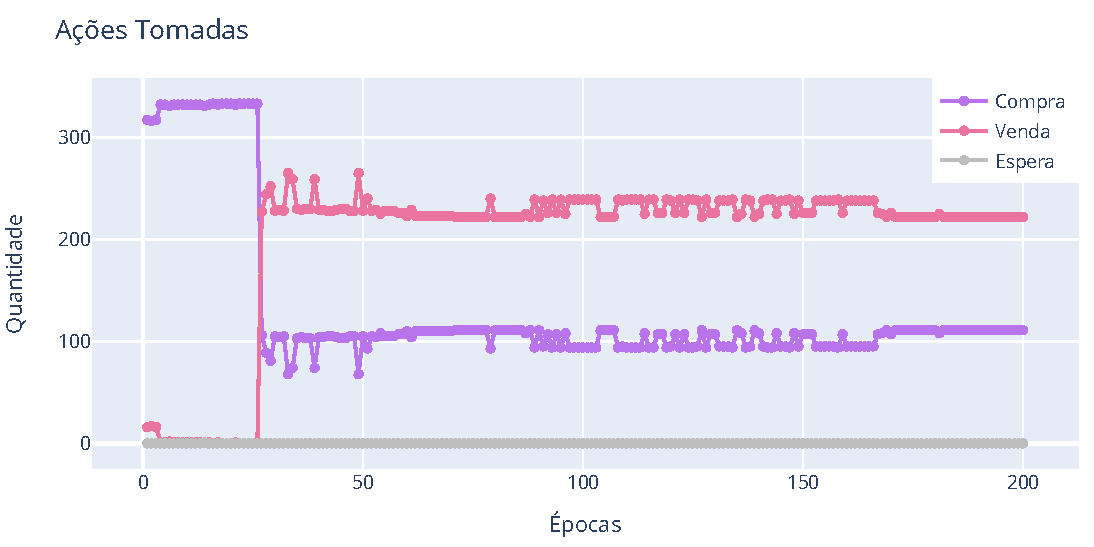
\includegraphics[width=\linewidth]{img/ddpg/all/clean/actions}
        \caption{Portfólio - Quantidade de ações selecionadas em teste.}
        \label{all_clean_act}
    \end{minipage}
\end{figure}

Portanto, nota-se que o modelo, apesar de todas as adversidades encontradas, obteve um lucro de R\$$5.874,00$ no final do teste, uma rentabilidade de $11,74\%$ no total dos 6 meses. A rentabilidade encontrada é $250,44\%$ maior que da poupança e $141,06\%$ maior que o \acrshort{CDI}. Nota-se que a rentabilidade encontrada é um pouco menor que a rentabilidade do ativo PETR3. Essa diferença pode ser justificada pelo fato do ativo da Petrobras ser o único que valoriza no período avaliado, sendo possível que o modelo entenda o risco de investir nos outros ativos. Com os resultados apresentados, responde-se positivamente as Perguntas \ref{peg3} e \ref{peg4} desse trabalho.

A análise do investidor seguindo uma estratégia \emph{buy and hold}, para essa situação demanda um estudo um pouco mais complicado. Essa complicação é devido ao fato de existir infinitas maneiras no qual um investidor pode montar seu portfólio com três ativos. Para o propósito desse trabalho, construiu-se um portfólio comparativo considerado ótimo, seguindo a teoria de Markowitz. O processo em construção desse portfólio leva em consideração a quantificação do retorno e o risco individual de cada ativo para posteriormente achar uma fronteira eficiente que tenha a maior possibilidade de retorno para a quantidade de risco que se deseja assumir.

\subsubsection{Análise Comparativa Com Fronteira Eficiente}

A \refFig{fronteira_port} apresenta as combinações de portfólios existentes em relação ao retorno esperado para o primeiro semestre de $2014$ e o risco assumido pelo mesmo. Para calcular esses valores, é utilizado como base os preços de fechamento mensais ajustado de cada ativo\footnote{Dados retirados do site: \url{http://finance.yahoo.com}}, de $2011$ a $2013$. Com os preços, calcula-se então os retornos e riscos mensais, informações utilizadas para compor a carteira. A cor de cada combinação de portfólio é respectiva a um indicador que ajuda a descobrir um ponto de equilíbrio entre risco e retorno, denominado Índice de Sharpe. Esse indicador mede o retorno excedente de uma aplicação financeira em relação a outra aplicação livre de risco. A aplicação livre de risco escolhida para calcular o índice, foi o retorno do \acrshort{CDI} no ano de $2013$ ($8,06\%$)\footnote{Dados retirados do site: \url{https://www.tororadar.com.br/}}, ano anterior ao que queremos estudar. 

\figura{img/fronteira}{Fronteira eficiente do portfólio PETR3, VALE3, ABEV3}{fronteira_port}{width=\linewidth}

Os diversos portfólios que foram gerados na \refFig{fronteira_port} são frutos da aplicação de um método que tem como objetivo gerar simulações aleatórias de forma massiva para encontrar um resultado aproximado da realidade, denominado método de Monte Carlo. A fronteira eficiente foi então encontrada com um conjunto de $25.000$ simulações aleatórias. Dentro da fronteira, qualquer portfólio selecionado será considerado ótimo (de maior retorno e menor risco). No entanto, para esse trabalho consideramos dois portfólios apenas, o de menor risco, e o de maior índice de Sharpe, representados respectivamente pelos marcadores verde e vermelho. A carteira de menor risco estima um retorno semestral de $1.18\%$, com um risco de $45\%$, sendo construída de $17.86\%$ PETR3, $42.91\%$ VALE3 e $39.22\%$ ABEV3. Por outro lado, a carteira de maior índice de Sharpe, possui um potencial de retorno de $4.28\%$ com um risco de $80\%$, sendo construída por $4.54\%$ PETR3, $0.1\%$ VALE3 e $95.36\%$ ABEV3.

Tendo a porcentagem de cada ativo para cada portfólio podemos então criar os portfólios em que um investidor alocaria seu saldo de R\$$50.000,00$. Começando pela estratégia mais segura, seguindo o portfólio de menor risco, o investidor distribuiria seu dinheiro nos ativos da forma supracitada. Relembrando, os preços iniciais dos ativos no período inicial de 2014 são R\$$15,01$ para PETR3, R\$$32,25$ para VALE3 e R\$$17,00$ para ABEV3. Nesses valores, o portfólio de menor risco, com os pesos resultantes da fronteira eficiente, consistiria de $500$ cotas da PETR3, $600$ cotas da VALE3 e $1100$ cotas da ABEV3, totalizando R\$$45.555,00$ investidos, e sobrando R\$$4.445,00$\footnote{Os valores selecionados para as quantidades de cotas são calculados com base na porcentagem de dinheiro que deve ser investido naquele ativo. Neste trabalho, consideramos que o agente não pode comprar ações fracionadas, apenas em lotes, portanto, a quantidade de cotas é sempre arredondada para a centena inferior.}. Os valores finais assumidos pelos ativos, no período analisado, foram de R\$$16,05$ para PETR3, R\$$29,06$ para VALE3 e R\$$15,54$ para ABEV3. Desta forma o investidor que seguir-se o portfólio de menor risco obteria um lucro de R\$$520,00$ na Petrobras, mas perderia R\$$1.914,00$ com a Vale e R\$$1.606,00$ com a Ambev. Obtendo um rendimento total de $-$R\$$3000,00$ do valor investindo e totalizando sua carteira com R\$$47.000,00$. O investidor que escolhesse pelo portfólio com maior índice de Sharpe seguiria por um caminho similar. Sua carteira seria alocada de $100$ cotas da PETR3, $0$ cotas da VALE3 e $2800$ cotas da ABEV3, totalizando R\$$49.101,00$ investidos, e sobrando R\$$899,00$ de saldo. Este investidor ganharia R\$$104,00$ na Petrobras, R\$$0,00$ na Vale, e seria abatido por uma perda de $-$R\$$4.088,00$ reais na ABEV3. O mesmo perderia R\$$3.984,00$ do dinheiro investido, totalizando R\$$46.016,00$ reais na carteira. Os resultados obtidos são resumidos na \refTab{tab:fronteira}.


\tabela{Comparação dos resultados obtidos pelo portfólio Hare com portfólios de fronteira eficiente}{tab:fronteira}{cc|c|c|}{
\cline{3-4}
                                                                                                                      &                                                                            & Valores Estimados & Valores Reais \\ \hline
\multicolumn{1}{|c|}{\multirow{2}{*}{\begin{tabular}[c]{@{}c@{}}Portfólio de Maior \\ Índice de Sharpe\end{tabular}}} & Lucro                                                                      & R\$$2.140,00$      & $-$R\$$3.984,00$   \\ \cline{2-4} 
\multicolumn{1}{|c|}{}                                                                                                & Rentabilidade                                                              & $4,28\%$          & $-7,96\%$       \\ \hline
\multicolumn{1}{|c|}{\multirow{2}{*}{\begin{tabular}[c]{@{}c@{}}Portfólio de \\ Menor Risco\end{tabular}}}            & Lucro                                                                      & R\$$590,00$          & $-$R\$$3.000,00$   \\ \cline{2-4} 
\multicolumn{1}{|c|}{}                                                                                                & Rentabilidade                                                              & $1,18\%$          & $-6\%$        \\ \hline
\multicolumn{1}{|c|}{\multirow{4}{*}{\begin{tabular}[c]{@{}c@{}}Portfólio do\\ Hare\end{tabular}}}                    & Lucro                                                                      & \textbf{-}        & R\$$5.874,00$ \\ \cline{2-4} 
\multicolumn{1}{|c|}{}                                                                                                & Rentabilidade                                                              & \textbf{-}        & 11,74\%     \\ \cline{2-4} 
\multicolumn{1}{|c|}{}                                                                                                & \begin{tabular}[c]{@{}c@{}}Rendimento Comparado \\ à Poupança\end{tabular} & \textbf{-}        & $250,44\%$    \\ \cline{2-4} 
\multicolumn{1}{|c|}{}                                                                                                & \begin{tabular}[c]{@{}c@{}}Rendimento Comparado\\ ao CDI\end{tabular}      & \textbf{-}        & 141,06\%   \\ \hline
}

O primeiro semestre de 2014 não viria a ser um período lucrativo para um investidor que seguisse o modelo de composição de portfólio baseados na fronteira eficiente. Os portfólios de menor risco e maior índice de Sharpe que possuíam capacidades para apresentar retornos de $1,18\%$ e $4,28\%$, sucumbiram a seus riscos, fornecendo uma rentabilidade real de $-6\%$ e $-7,96\%$. Portanto, o investidor que seguisse o modelo treinado com o \acrshort{DDPG} proposto pelo Hare, obteria no final dos $6$ meses uma rentabilidade de $11,74\%$, um retorno claramente maior que os retornos reais e projetados dos portfólios considerados ``eficientes''. Demonstrando assim, a viabilidade do modelo proposto para investimentos na bolsa de valores, e respondendo à Pergunta \ref{peg5} proposta.

\section{Considerações Finais}
\label{exp:consideracoes}

Este capítulo realizou a validação do serviço proposto em duas etapas, primeiro validando o \acrshort{MPM}, seguindo com a validação o \acrshort{MAR}. Para tanto, criou-se uma rotina de exploração de hiper-parâmetros e treinou-se os modelos que obtiveram os melhores desempenho. Os dados obtidos demonstraram resultados satisfatórios para os modelos gerados, com acurácia de até $92.0\%$ no ativo PETR3, $82\%$ em VALE3, e $94\%$ em ABEV. Tais resultados foram comparados, avaliando o desempenho em relação aos modelos tradicionais da literatura. O modelo proposto obteve a maior acurácia e a maior média das métricas obtidas. Posteriormente, realizou-se a validação do \acrshort{MAR}, começando pelos ativos individuais até chegar no portfólio completo. Os resultados obtidos, mostraram uma rentabilidade de $13,77\%$ em PETR3, $6,03\%$ em VALE3, $0\%$ em ABEV, e $11,74\%$ para o portfólio completo. O resultado do portfólio foi comparado com um ``portfólio eficiente'' criado utilizando a \acrshort{VMM}, obtendo resultados consideravelmente melhores, visto que o ``portfólio eficiente'' apresentaria perdas no fim do período analisado.
 
Os experimentos realizados no algoritmo \acrshort{DDPG} envolveram muitas tentativas (e erros), nos quais não foram mencionados. Diversas funções de recompensas foram testadas, estas incluem: valores simples como $-1$ e $+1$ para recompensas de perda ou lucro respectivamente, valores de recompensa somente no fim da simulação, recompensas baseadas em ganho diário, dentre diversas outras. Nenhuma das recompensas apresentou um resultado tão eficiente quanto o demonstrado, muita das vezes convergindo para uma política especifica na primeira época e não explorando. Acredita-se que o \acrshort{DDPG} possa estar apresentando dois principais problemas à formulação da função recompensa: recompensas esparsas e falta de reforços positivos. Esses dois casos podem estar levando o \acrshort{DDPG} a uma situação de \emph{deadlock}, onde não consegue mais aprender \cite{matheron2019problem}. Além das funções de recompensa, espaço de estados diversos também foram implementados, variando o espaço de estados apresentados no desenvolvimento, incluindo situações onde o espaço de estados possuía somente o indicador de movimento. Nenhum dos quais apresentaram resultados demonstráveis. Ademais, notou-se que o \acrshort{DDPG} é extremamente sensível a hiper-parametrização, desde a semente aleatória que gerará o modelo até o tamanho da camada escondida, diversos parâmetros foram testados, os apresentados neste trabalho foram os que obtiveram melhores resultados.